\cleardoublepage
\chapter{Planlegging av produktet}
\label{chap:design} 
% \meta{
%  Basert på beskrivelsen av oppgaven (Avsnitt \ref{sec:oppgaven}) og analysen i (Kapittel \ref{chap:analysis}), skal denne delen beskrive hvordan man har tenkt å utforme løsningen. Beskrivelsen er noe avhengig av type prosjekt.

% \paragraph{Utredning}

% Først og fremst må det redegjøres for hvordan man skal innhente informasjonen som skal danne grunnlaget for utredningen. Deretter må man bestemme hvordan man skal behandle materialet, f.eks. om man skal bruke statistiske metoder. Etter det er det naturlig å presentere en disposisjon for selve utredningen, som i dette tilfellet vil være hovedresultatet i prosjektet. Selve utredningen bør være et frittstående dokument, på samme måte som en film vil være et frittstående dokument i en mediaproduksjon, og et program vil være i et utviklingsprosjekt.

% \paragraph{Mediaproduksjon}
% Her vil det være naturlig å presentere story-boards og liknende metoder for å beskrive produksjonen. 

% \paragraph{Utvikling}
% Her er det bare å ta for seg av ulike måter å beskrive systemer på, alt fra overordnet arkitektur, moduler, meldingsprotokoller etc. Bruk gjerne formelle beskrivelsesspråk, typisk UML. 
% }

% I det videre tar vi for oss oppgaven med å utvikle struktur, innhold og formgiving av rapportmalen, uavhengig av hvilket verktøy som skal brukes ved implementasjonen.



% ---

I dette kapittelet vil vi ta for oss hvordan vi har tenkt å utforme nettstedet. Vi vil presentere forslag til innhold, struktur, design, utforming av CMS og databaser. Dette vil være grunnlaget for resten av oppgaven.

% Sirkus Media "Vi vet ikke helt hva vi vil ha før vi ser det". Samtale 27.02.2019.

% \section{Strategi og planlegging}
% I alle type prosjekter er det viktig å ha en strategi og planlegge etter dette, og det kan være helt avgjørende å ha en god plan.

% Når det kommer til webdesign-prosjekter inneholder disse fire viktige komponenter. Første steg er at du må kjenne miljøet ditt. Andre steg er å planlegge. Tredje steg er å lære å kunne tilpasse seg, og siste steg er å fullføre prosessen ved å løse kompatibilitetsproblemer etter hvert som de oppstår. (Dawson, 2011).

% Dawson, A. (2011). Future-proof web design. Retrieved from https://ebookcentral.proquest.com

% \url{https://www.sciencedirect.com/science/article/pii/S014829631630203X#bb0175 }


% ---

% \section{Struktur}

% Vi tar utgangspunkt i den tradisjonelle og generiske strukturen beskrevet i Avsnitt \ref{sec:mayfield}. Det er etter min mening vanskelig å se noen grunn til å gjøre noe annet.


\section{Planlegging av struktur og innhold}
\label{sec:planning-website}

Etter analysen gjort i kapittel \ref{chap:analysis} har studentgruppen kommet frem til at struktur og innhold burde være som følgende: 

\textbf{Forside} Tanken er at hele nettstedet i hovedsak skal bestå av en lang forside. Da dette ikke er beste praksis for søkemotoroptimalisering, vil vi forbedre SEO ved å lenke til nye sider som er mer detaljert. Høyt oppe på siden skal det være en knapp til et kontaktskjema. Telefonnummeret til bedriften skal også være lett tilgjengelig. I tillegg skal forsiden bestå av en beskrivelse av bedriften, presentasjon av hva de tilbyr og steg for steg om prosessen. Videre skal nettstedet ha et kart som er integrert med Google Maps og viser lokasjonen til bedriften. Nederst på nettstedet skal organisasjonsnummer, link til personvern og logg inn til CMS-et bli presentert.

\textbf{Meny} Nettstedets meny skal være tilgjengelig uavhengig av hvilken side brukeren står på. Her skal alltid forside, om oss og kontakt oss være tilgjengelig. 

\textbf{Om oss} Det vil også bli opprettet en egen \q{Om oss}-side som er tilgjengelig via menypunktet \q{Om oss}. Denne siden inneholder en mer detaljert presentasjon av Sirkus Media og deres visjon.

\textbf{Kontakt oss} Nettstedet vil i tillegg til kontaktskjema på forsiden, bestå av en egen side med kontaktinformasjon. Her presenteres også relevant informasjon som bedriftens adresse, e-post, mobilnummer og kart. Vi lager en dedikert side for kontaktinformasjon fordi det er positivt med tanke på søkemotoroptimalisering. For eksempel: Hvis en bruker søker på Google etter Sirkus Media og det ikke er en egen side for kontakt oss, vil brukeren kun få treff på forsiden og undersidene med andre irrelevant temaer. Siden brukeren ønsker å kontakte Sirkus Media, er det mer brukervennlig å ha en link til kontakt siden i Google.

\textbf{Logg inn} Dette er en egen side der de ansatte kan logge inn for å komme til brukergrensesnittet for oppdatering og endring av innhold.

\textbf{Administrasjonsside}  På administrasjonssiden kan de ansatte endre og legge til innhold gjennom et brukergrensesnitt.

\textbf{Informasjon om personvern og informasjonskapsler} Personvernsiden skal inneholde en personvernserklæring. Denne forteller hvordan Sirkus Media samler inn og bruker personopplysninger. Målet er å gi brukerne overordnet informasjon om deres behandling av personopplysninger. I tillegg skal den fortelle brukeren hvilke informasjonskapsler som blir brukt på nettstedet.

\textbf{Annet} Alle sidene skal ha tilgang til en chat, der det er mulig å ta direkte kontakt med bedriften.

\section{Definering av CMS}
\label{sec-planning-cms}
Etter å ha planlagt innholdet måtte gruppen sette seg ned og bestemme hvordan systemet skulle fungere. I felleskap kom vi frem til følgende:

\begin{itemize}
\item CMS-et skal bestå av flere sider (pages).
\item Hver side inneholder en eller flere komponenter (components), som er gjenbrukbare biter av kode, og kan tilhøre flere sider.
\item Hver komponent inneholder felter (fields), som holder på innholdet som vises på siden. Det er forskjellige type felter, for eksempel kan et felt være et bilde, et tekstområde eller en lenke. 
\end{itemize}

Videre ble det bestemt at studentgruppen, eller en fremtidig superadmin, ferdigdefinerer komponenter og felter. I brukergrensesnittet til back-end vil oppdragsgiver få mulighet til å opprette sider med ønsket komponenter og felter.  


\section{UML-diagram}
Figur \ref{fig:database} viser databasen som ble planlagt for prosjektet:
\begin{figure}[H]
    \centering
    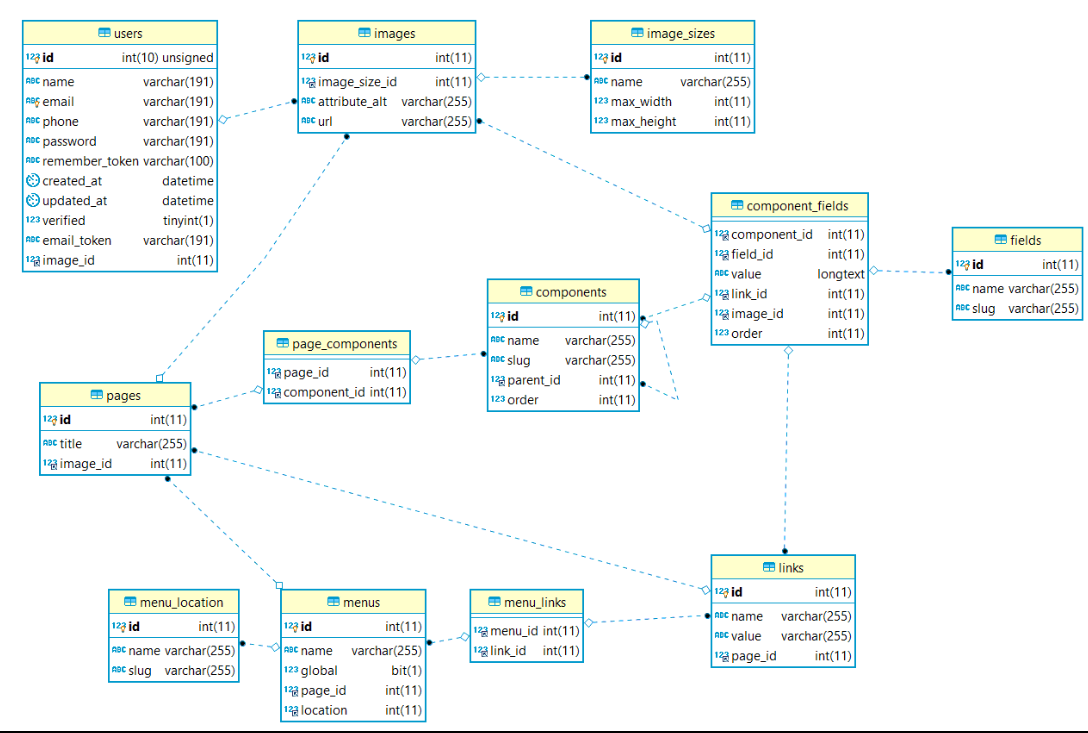
\includegraphics[width=\textwidth]{planlegging-av-database.png}
    \caption{Prosjektets planlagte database}
    \label{fig:database}
\end{figure}


\subsection{Planlegging av API URL-er}
I felleskap begynte vi å planlegge hvilke linker som API-et skal ha, og hva de skal sende i svar. Det ble derfor utarbeidet en JSON-fil som beskriver strukturen og hvilke data den skal gi i svar for forskjellige forespørsler.

I første omgang ble URL-er for Pages og Menus definerte. Dataene disse gir i svar, vil være offentlig. 

Slik så JSON filen ut når Pages og Menus var definert:
--- PUTT JSON FIL HER ---

Denne filen er altså kun eksempeldata. Den vil bli brukt til å se på at back-end sender svar på riktig måte. Front-end kan også se på filen for hvilke svar som kan forventes på de forskjellige forespørselene. Fordelen med dette er at det kan lages dummy responses som er mulig å jobbe med underveis i utviklingen.

\section{Mockups}
En del av planleggingsfasen var å lage mockups/skisser av nettstedet. Dette ble laget for forsiden, slik at skissene kunne sendes for å få godkjenning av oppdragsgiver.

Mockupene ble utarbeidet av Bjørnar. 

\subsection{Versjon 1}
Figur \ref{fig:mockup-v1} viser forsøk nummer 1. Tilbakemeldingen her var oppdragsgiver syns det var et kult design, men ikke helt den stilen de ønsket seg.
\begin{figure}[H]
    \centering
    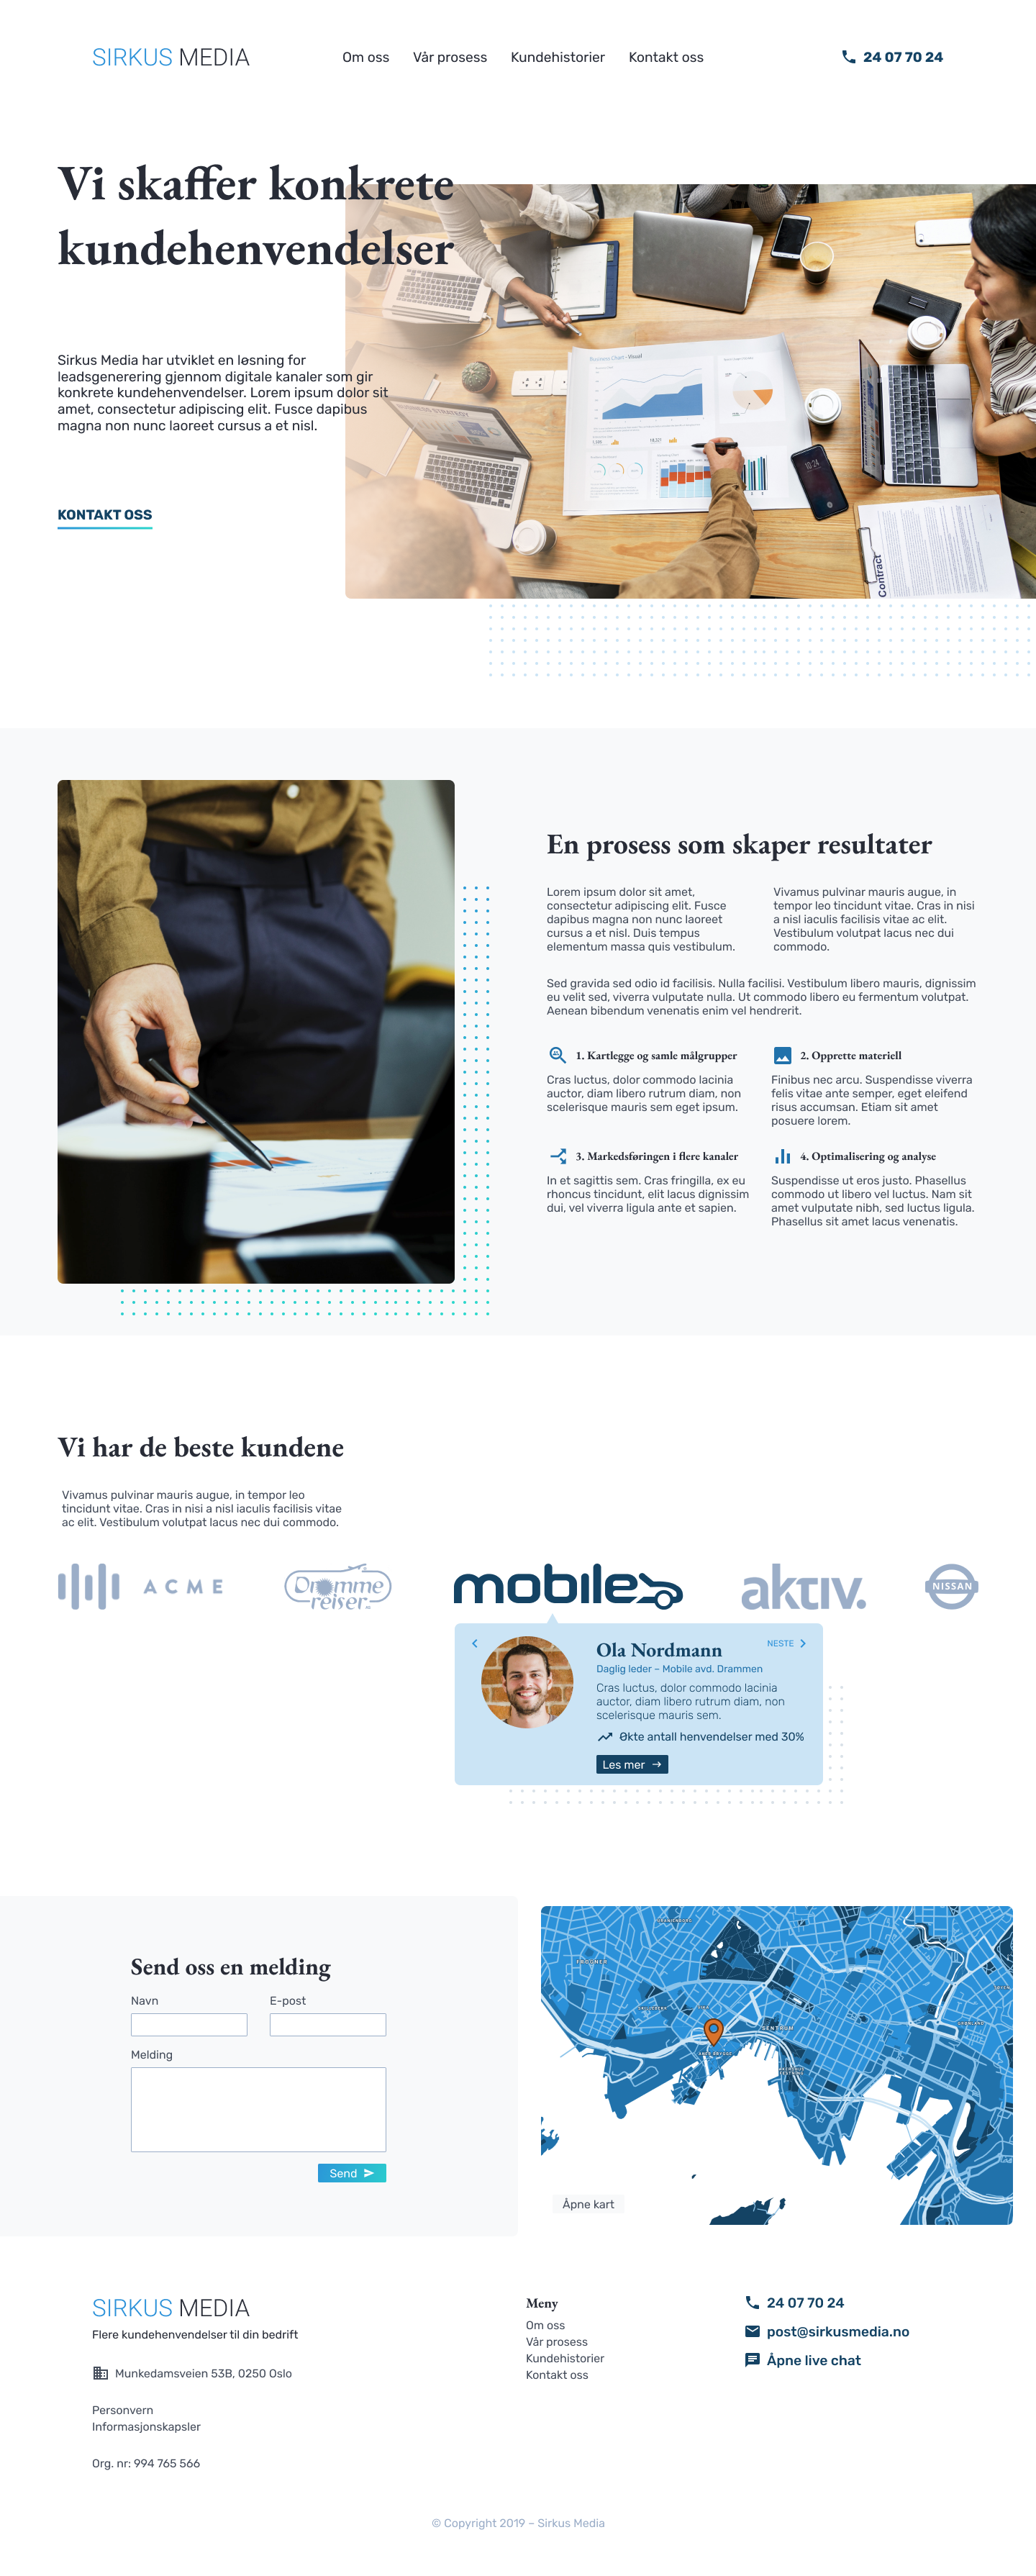
\includegraphics[height=\textheight]{mockup1-draft3.png}
    \caption{Mockup - Versjon 1}
    \label{fig:mockup-v1}
\end{figure}

\subsection{Versjon 2}
Figur \ref{fig:mockup-v2} viser forsøk nummer 2. Tilbakemeldingen her var den samme som på versjon 1.
\begin{figure}[H]
    \centering
    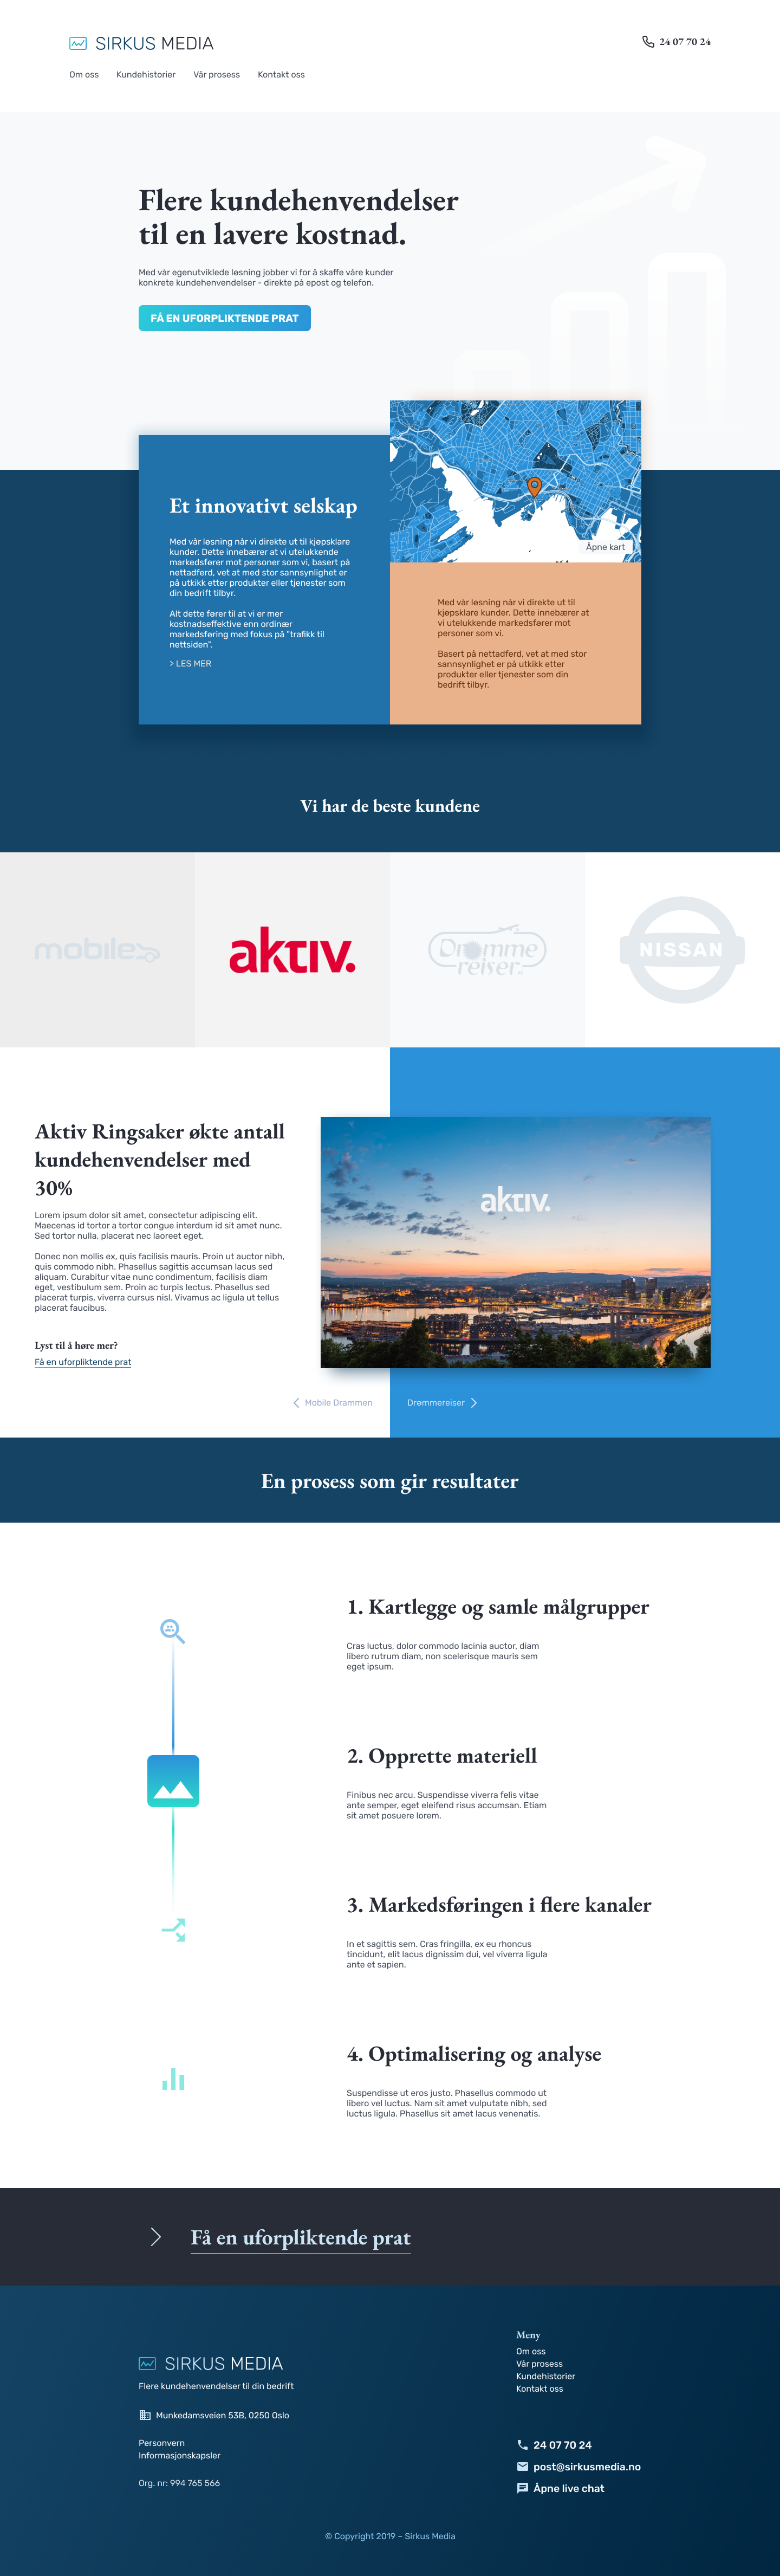
\includegraphics[height=.85\textheight]{mockup2-draft3.png}
    \caption{Mockup - Versjon 2}
    \label{fig:mockup-v2}
\end{figure}

\subsection{Versjon 3}
Figur \ref{fig:mockup-v3-index} viser det tredje forsøket. Dette var skissen som ble godkjent.
\begin{figure}[H]
    \centering
    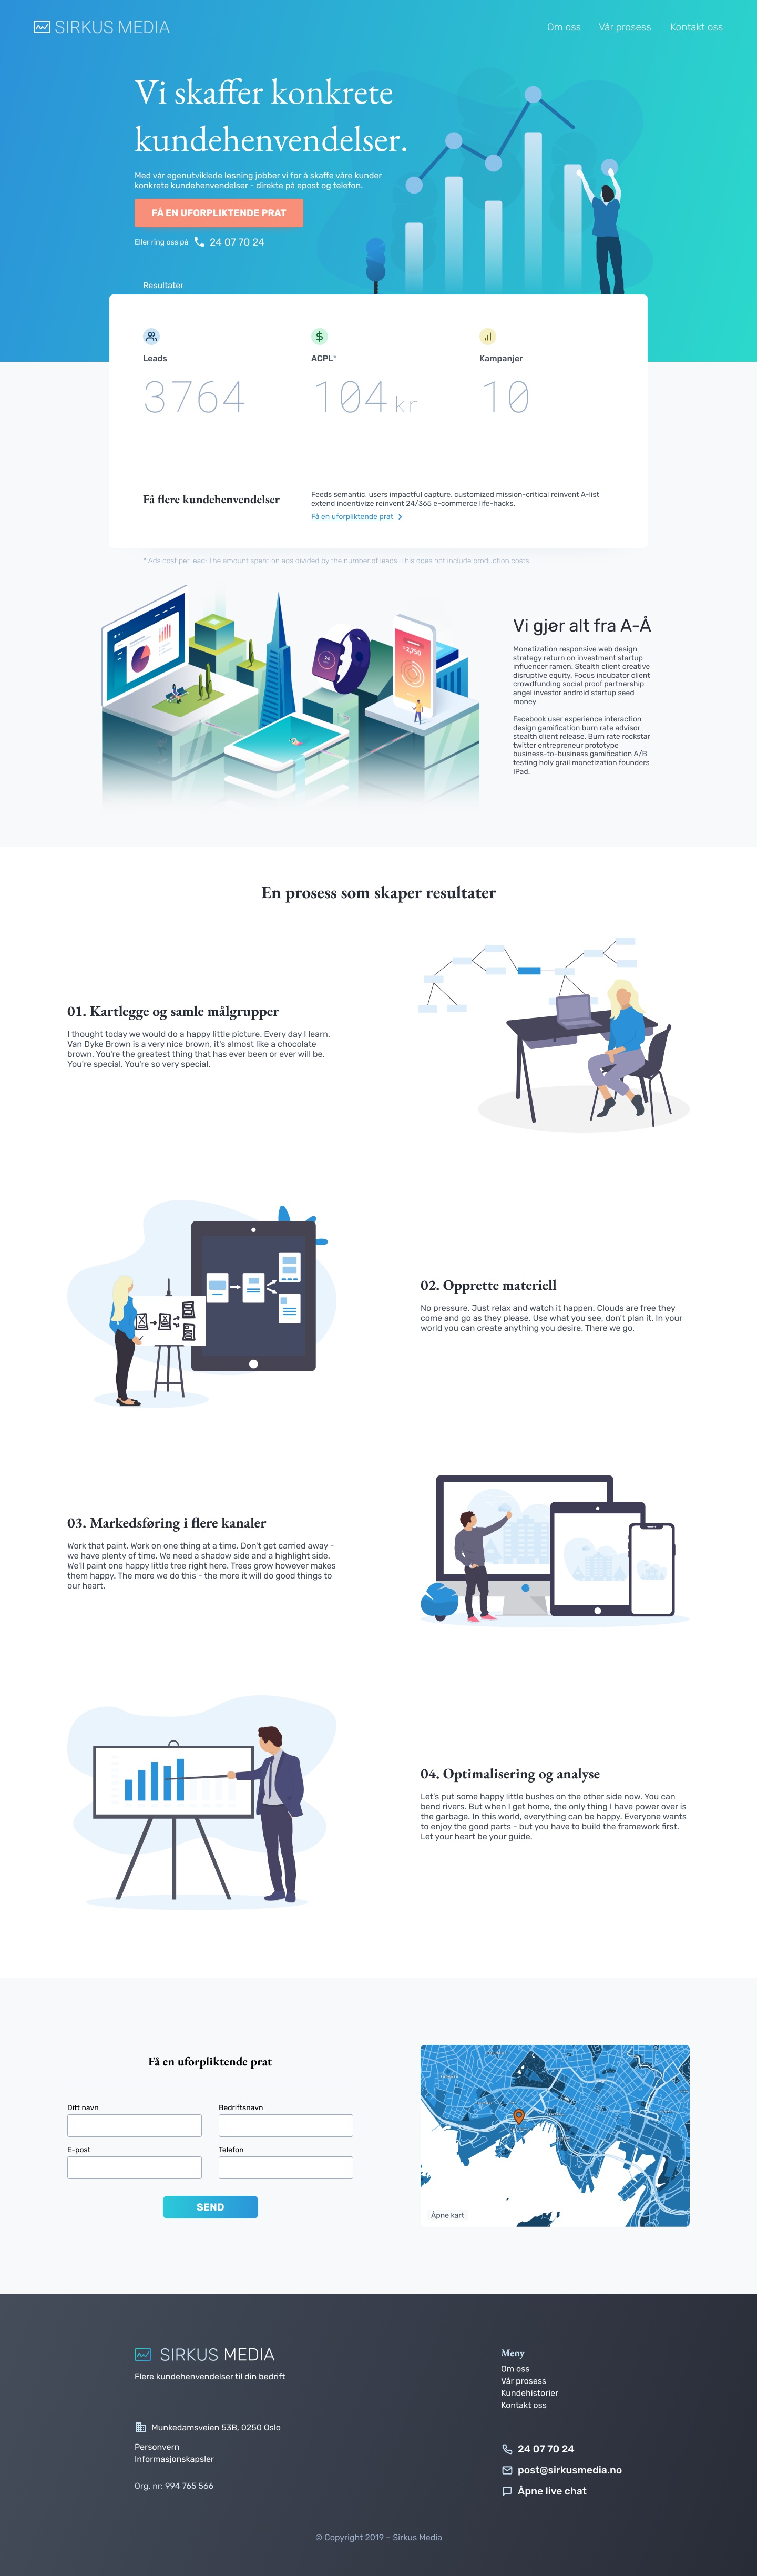
\includegraphics[height=.82\textheight]{mockup3-index.png}
    \caption{Mockup - Versjon 3 - Forside}
    \label{fig:mockup-v3-index}
\end{figure}

Når designet til forsiden ble godkjent, startet utarbeidingen av designet til de andre planlagte sidene på front-end.

\textbf{Om oss}
Figur \ref{fig:mockup-v3-about} viser designet til den planlagte \q{Om oss}-siden.
\begin{figure}[H]
    \centering
    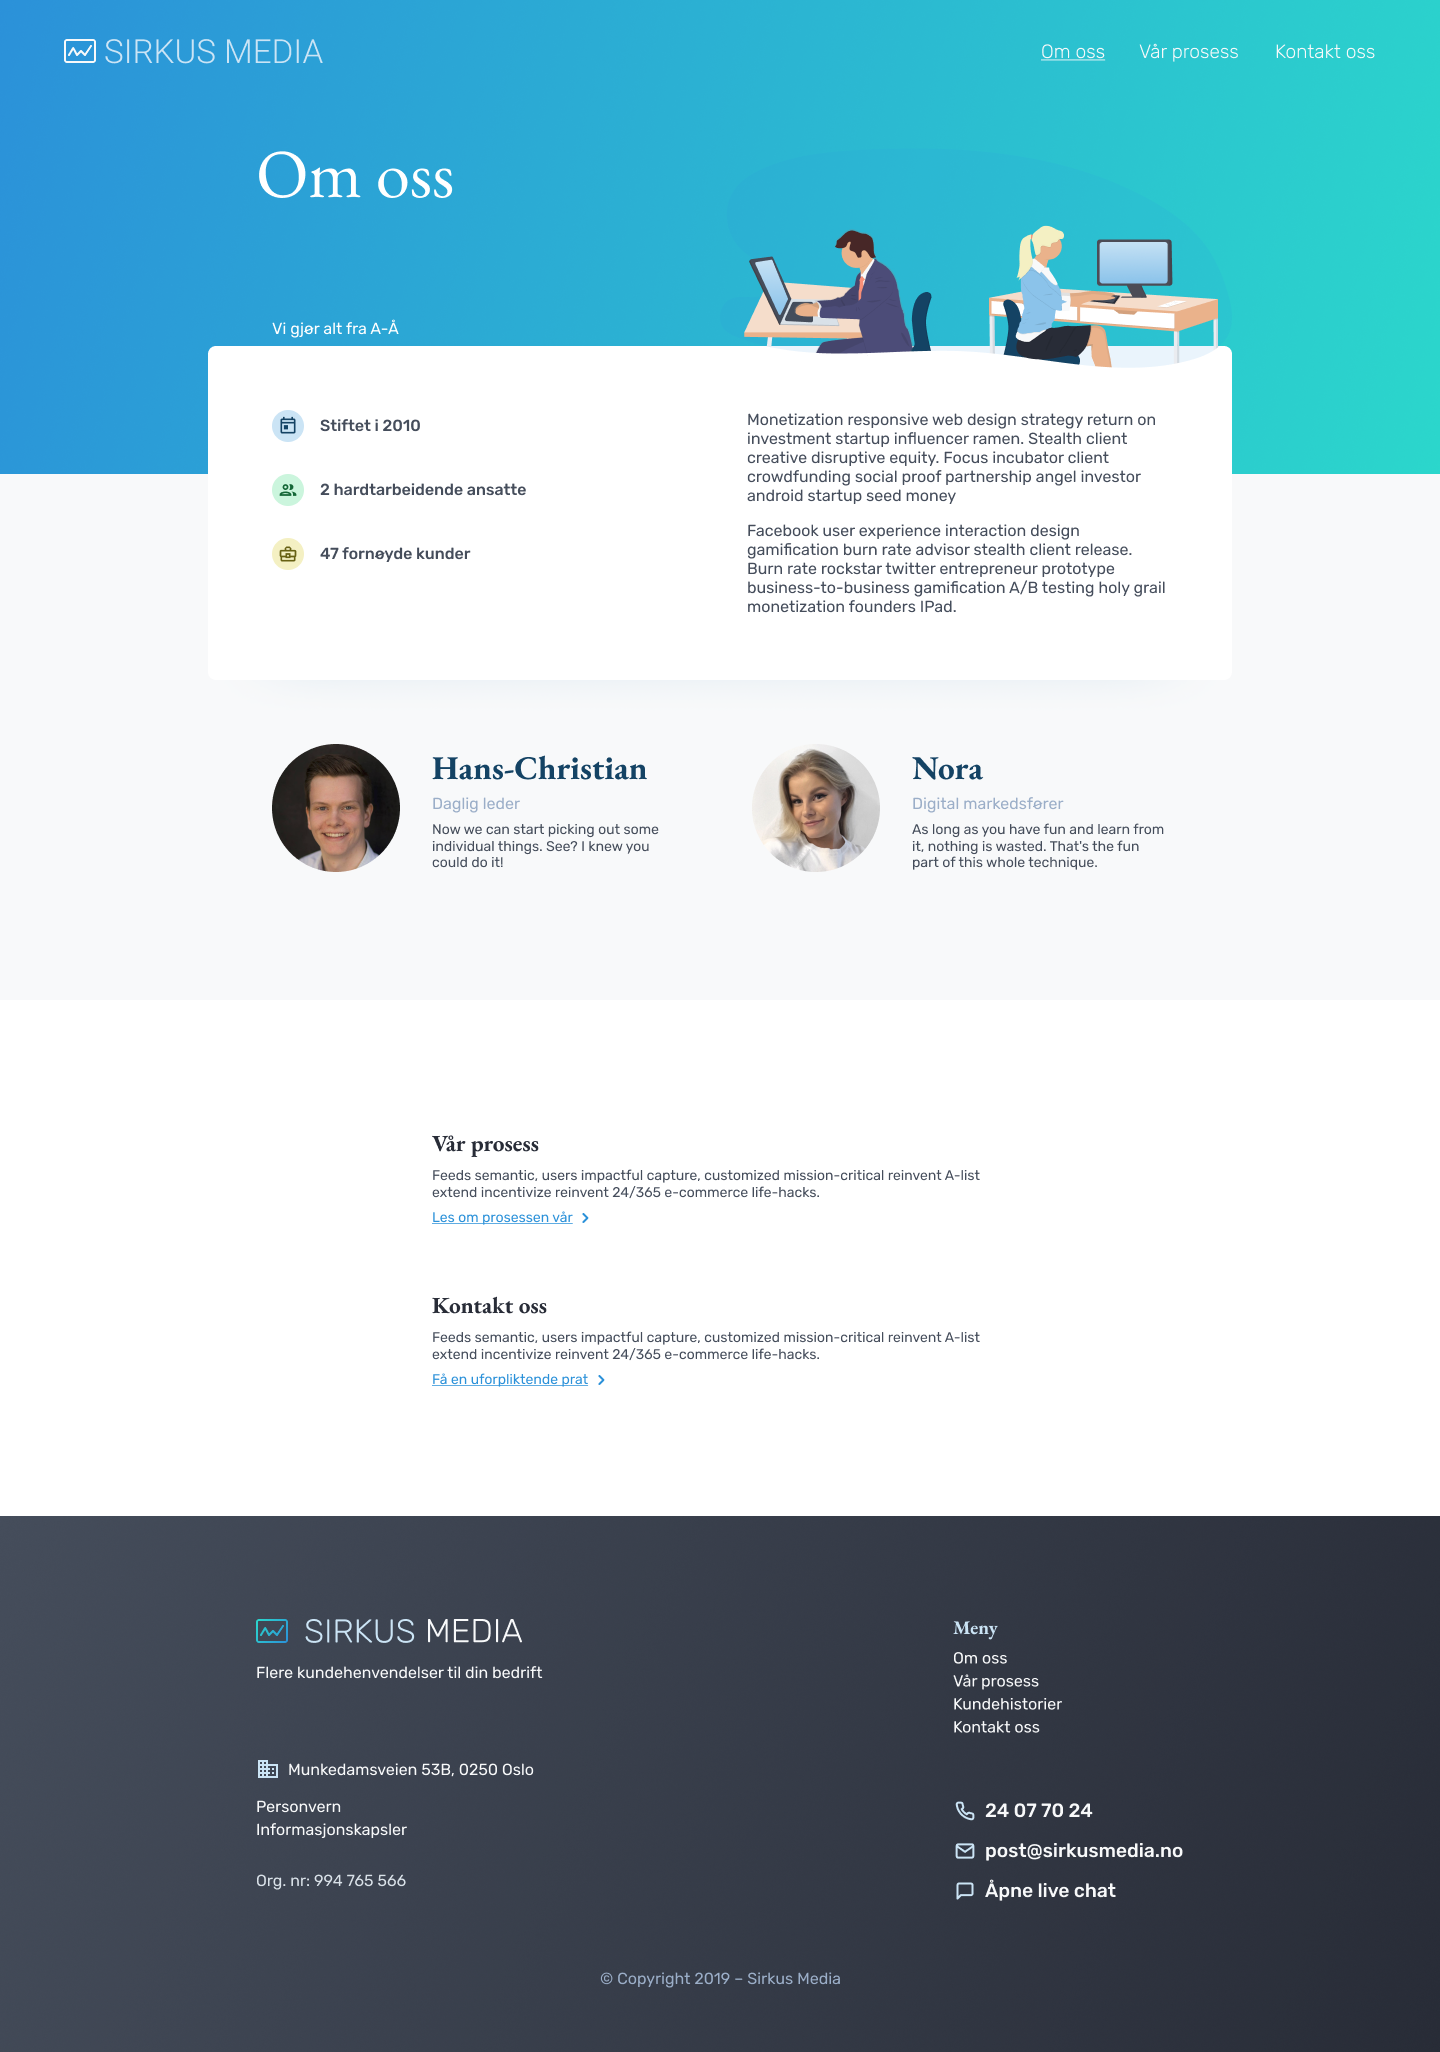
\includegraphics[height=.9\textheight]{mockup3-about.png}
    \caption{Mockup - Versjon 3 - Om oss}
    \label{fig:mockup-v3-about}
\end{figure}

\textbf{Kontakt oss}
Figur \ref{fig:mockup-v3-contact} viser designet til den planlagte \q{Kontakt oss}-siden.
\begin{figure}[H]
    \centering
    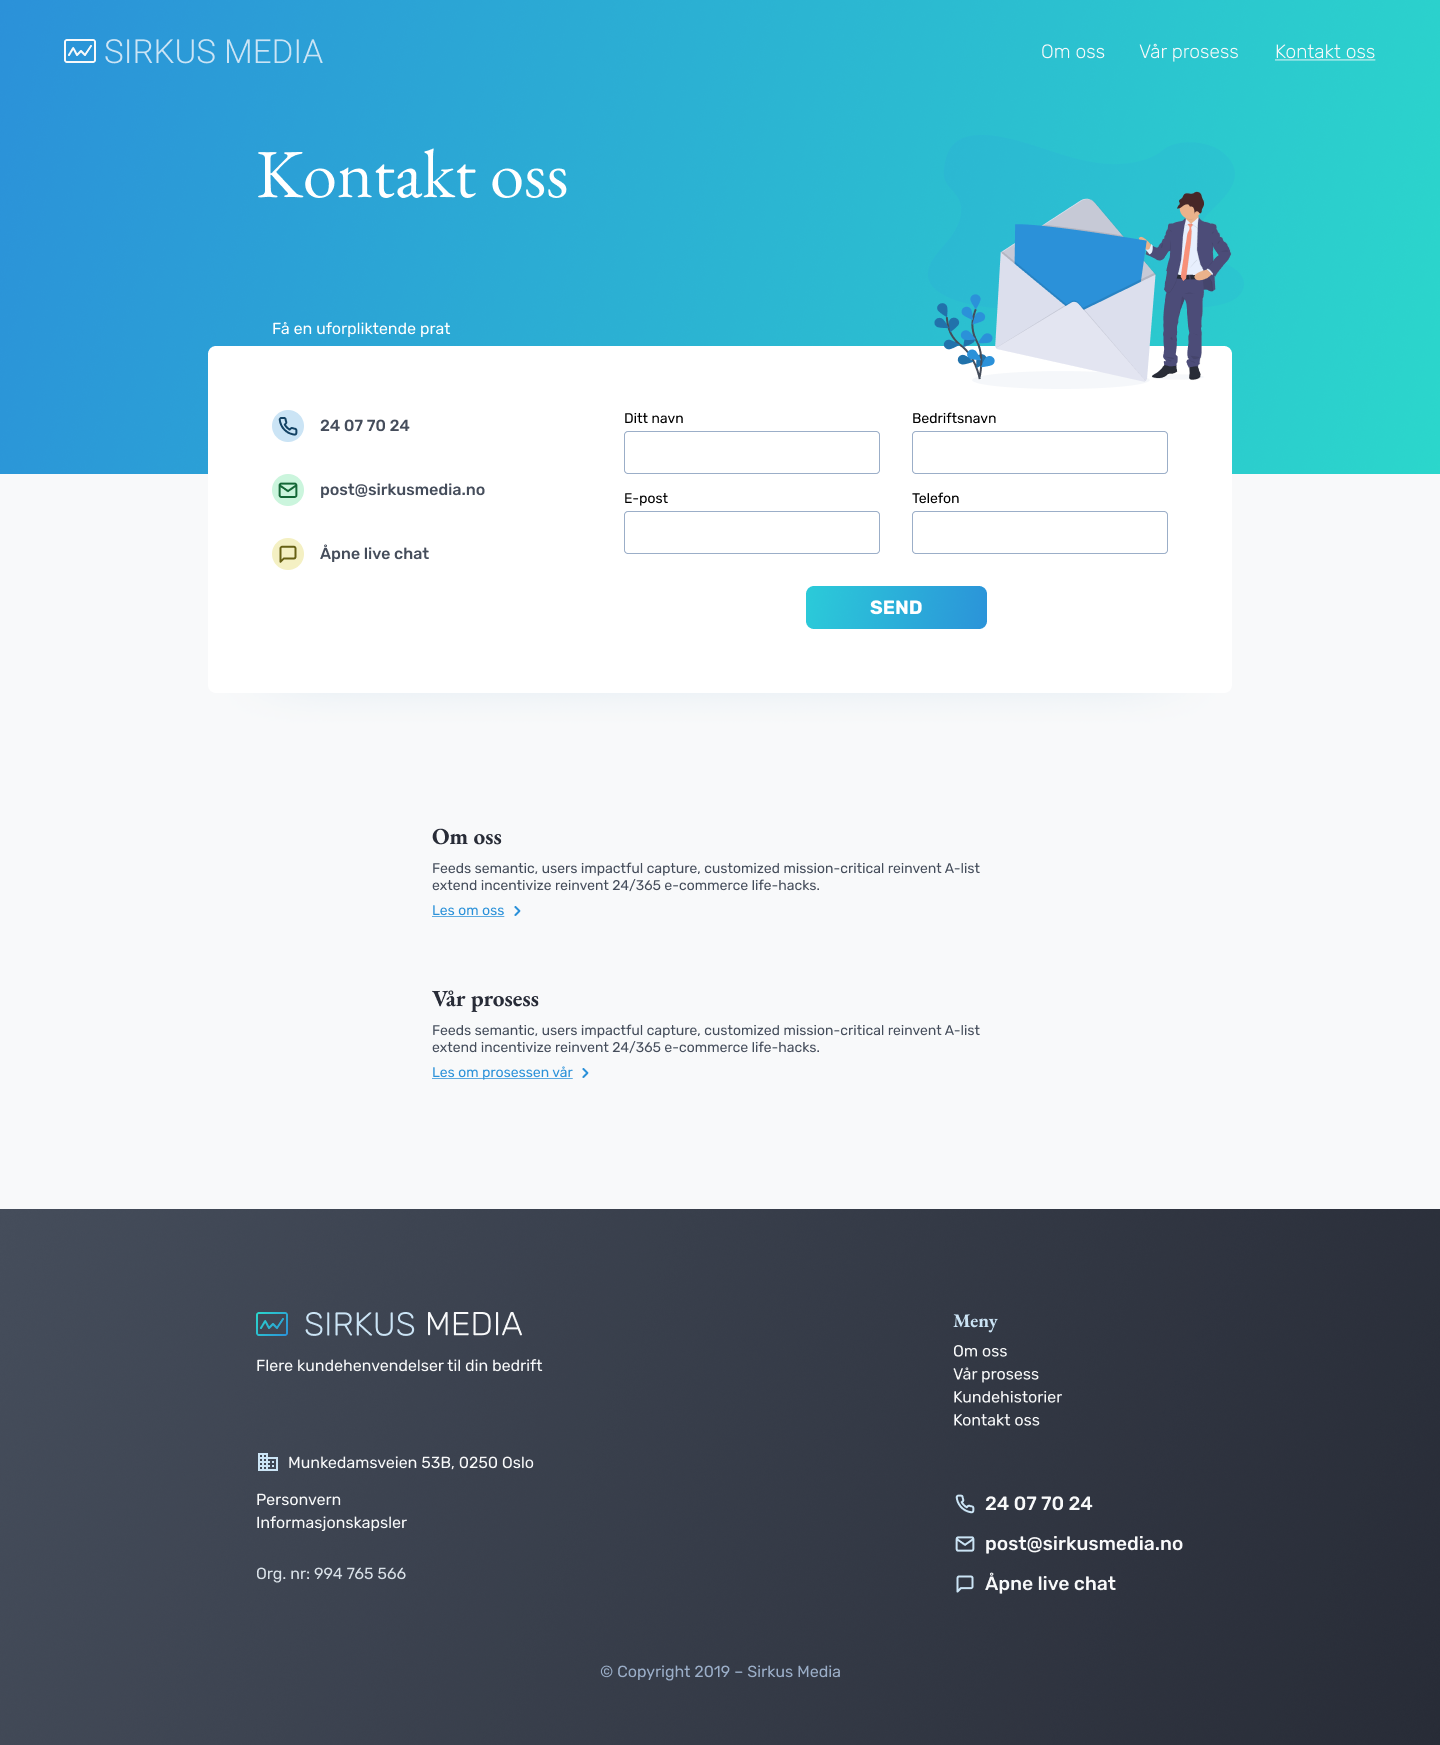
\includegraphics[width=\textwidth]{mockup3-contact.png}
    \caption{Mockup - Versjon 3 - Kontakt oss}
    \label{fig:mockup-v3-contact}
\end{figure}


\section{Visuell profil}
Videre ble det opprettet en enkel visuell profil for den godkjente skissen.

\subsection{Logo}
Figur .. viser logoen som ble utarbeidet.

\subsection{Farger}
Figur \ref{fig:colors} viser de utvalgte fargene til oppdragsgiver. Disse fargene ble valgt ut med tanke på å få selskapet til å fremstå som moderne og innovative.

\begin{figure}[H]
    \centering
    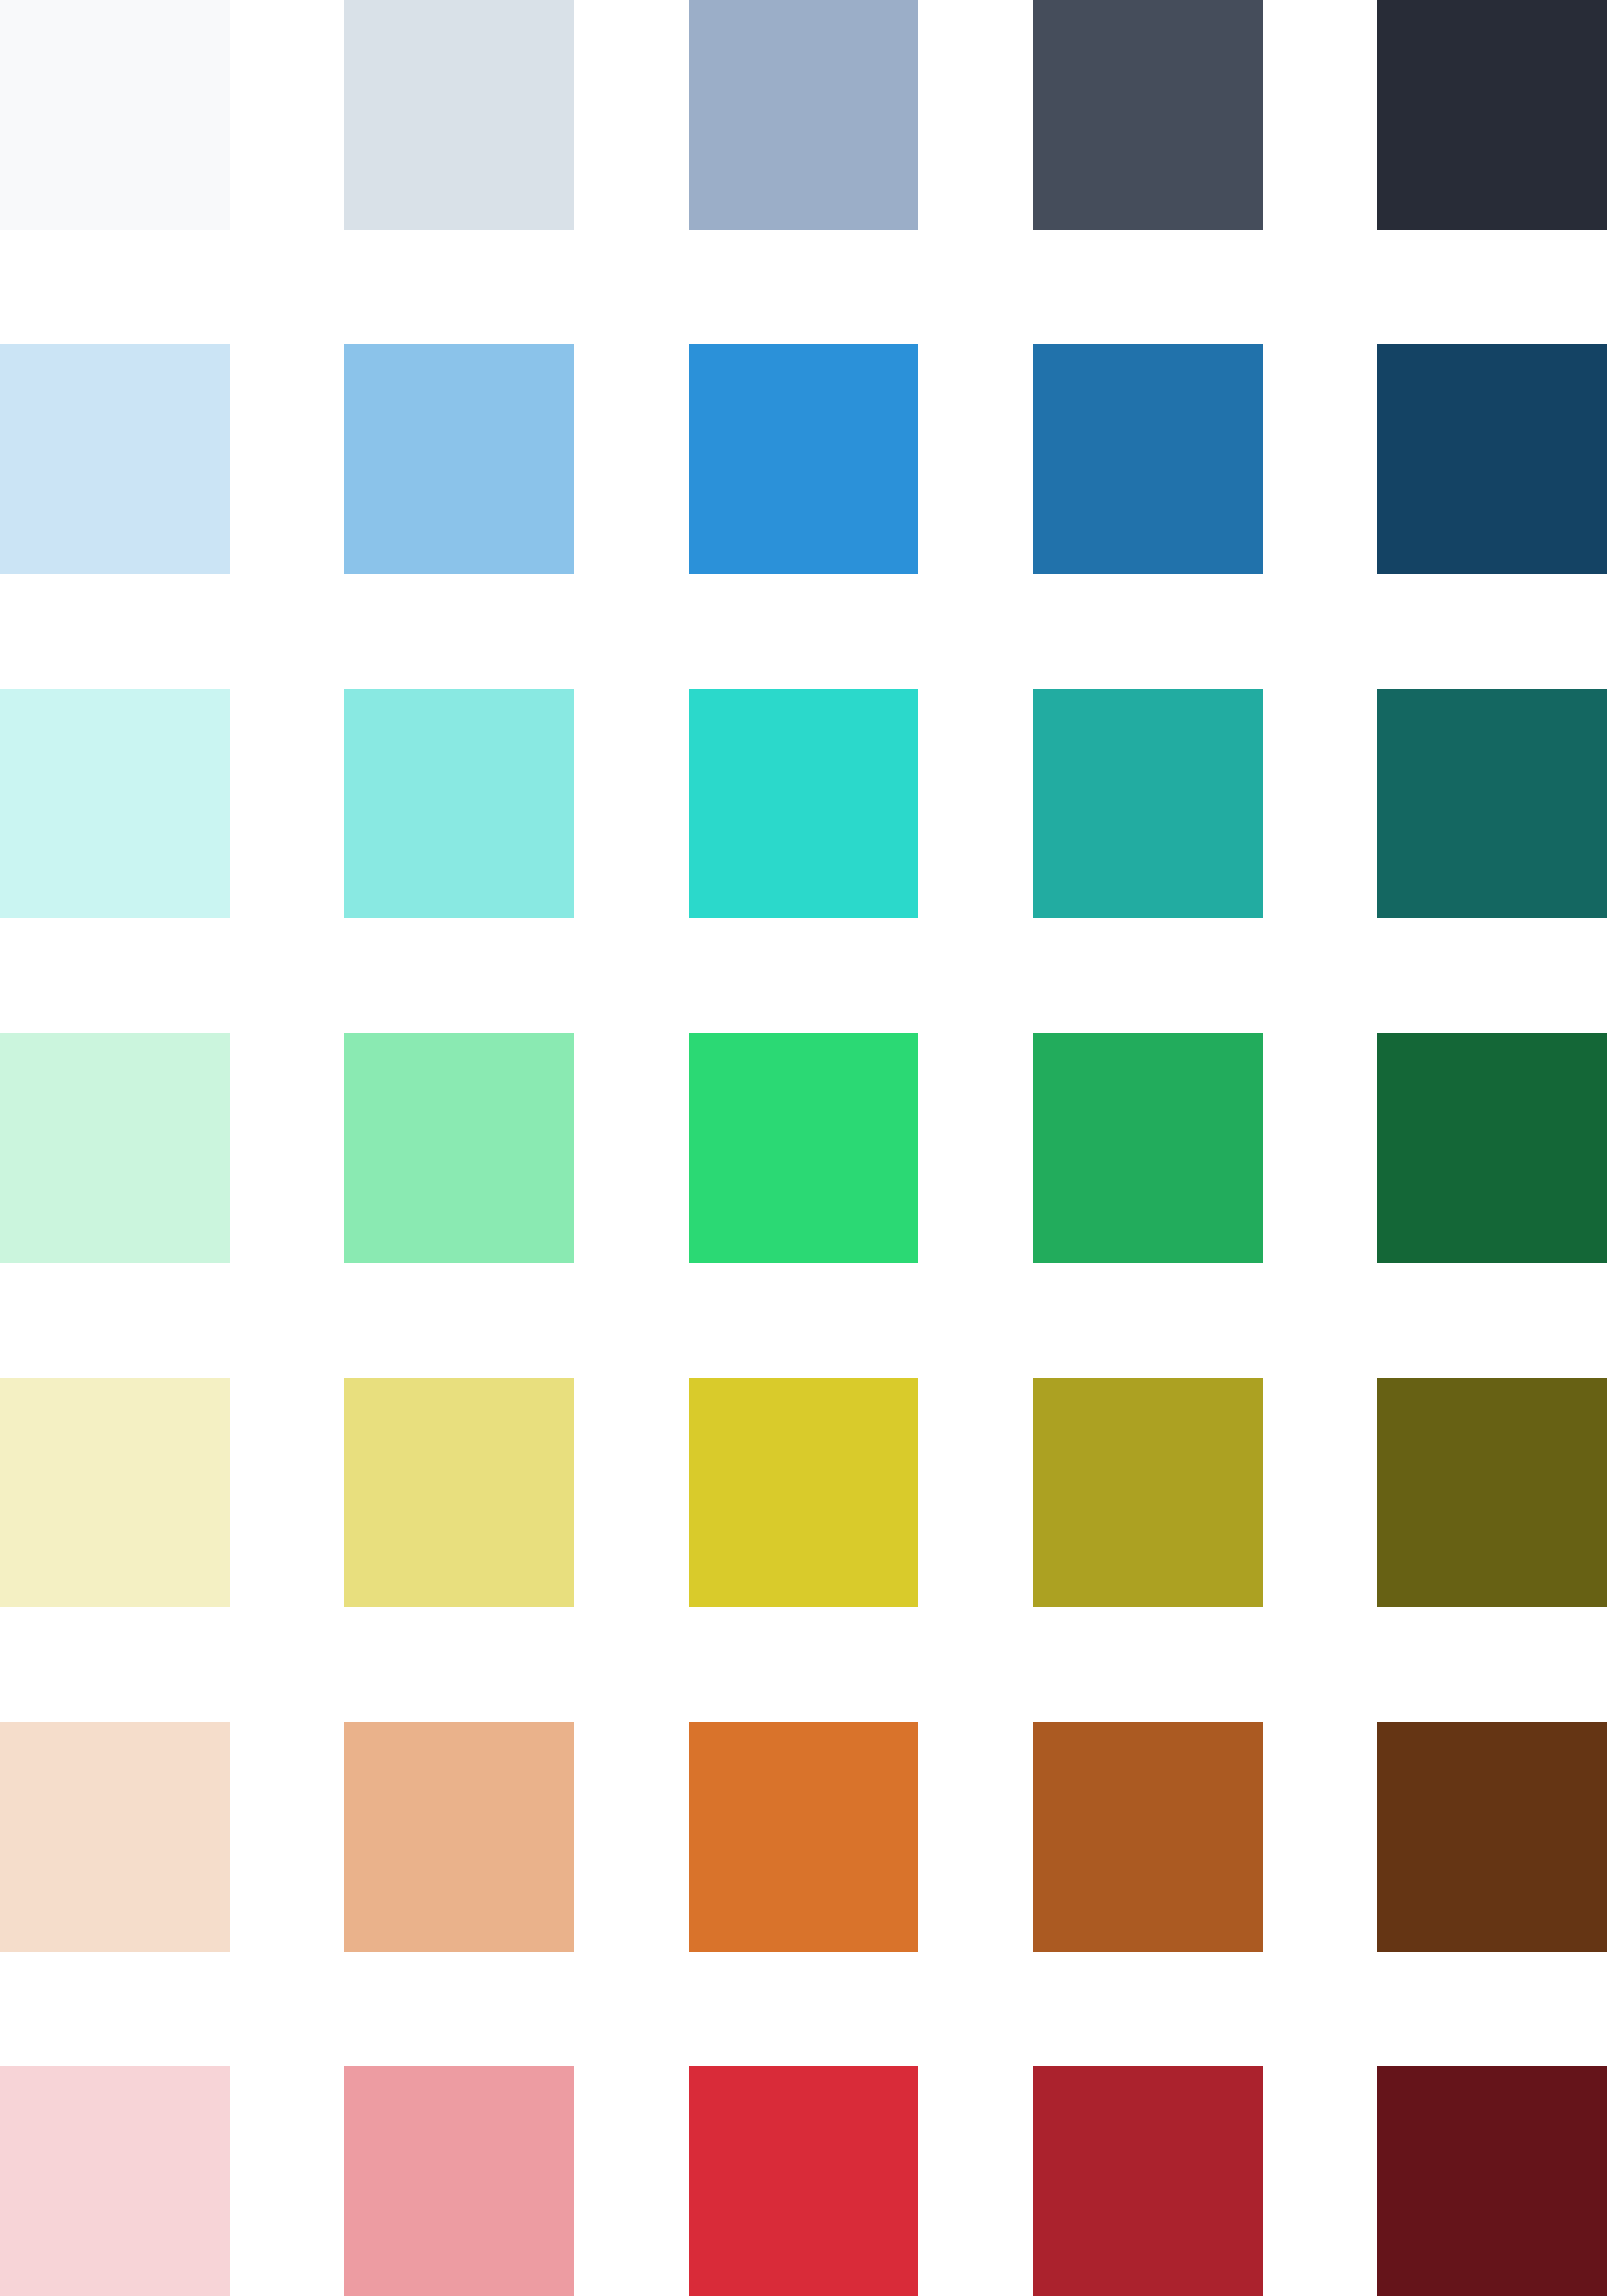
\includegraphics[width=.5\textwidth]{colors.png}
    \caption{Visuell profil - farger}
    \label{fig:colors}
\end{figure}

\subsection{Fonter}
Figur \ref{fig:typography} viser de utvalgte fontene til oppdragsgiver.

\begin{figure}[H]
    \centering
    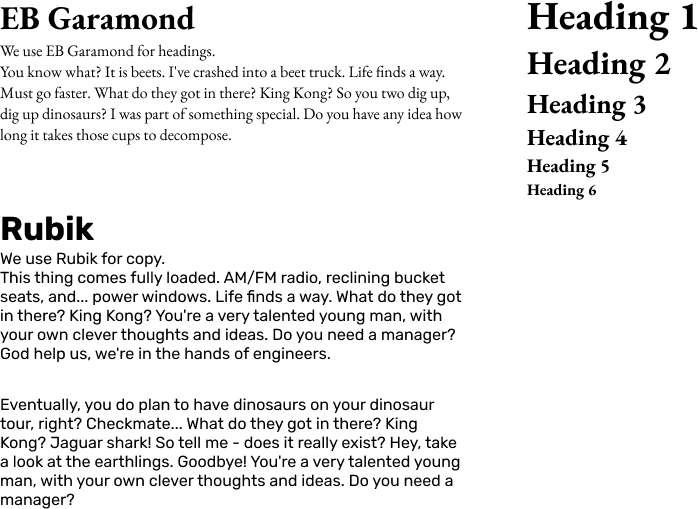
\includegraphics[width=\textwidth]{typography.png}
    \caption{Visuell profil - fonter}
    \label{fig:typography}
\end{figure}

% \section{Innhold}

% Vi så Avsnitt \ref{sec:hiof-it}  at man ved HiØ skiller mellom produkt- og prosessdokumentasjon, og operer med flere frittstående dokumenter. Det er ønskelig at hovedokumentet omhandler løsningen av oppdraget, dvs. selve produktet.
% Struktur og innhold bør være som som følger:

% \begin{compactdesc}
% \item [Front Matter]  Som i Avsnitt \ref{sec:mayfield}.

% \item [Body] Hoveddelen av dokumentet (gjennomføringen).
% \begin{compactdesc}
% \item [Introduksjon] Skal gi leseren et bilde av rammene rundt prosjektet: Kort beskrivelse av oppdraget, litt om oppdragsgiver og prosjektgruppen, prosjektets formål, leveranser og metoder. Den bør også inneholde en oversikt over resten av rapporten. 
% \item [Analyse] Kapittelet tar for seg analysedelen av arbeidet. Den består av to hoveddeler, en grundig beskrivelse av oppgaven basert på skissen gitt av oppdragsgiver, og en undersøkelse av hva som finnes av relatert arbeid, {\em best practise} og relevant teknologi. 
% \item [Design]  Basert på beskrivelsen av oppgaven i introduksjonen  og analysen, skal denne delen beskrive hvordan man har tenkt å utforme løsningen. Beskrivelsen er nødvendigvis noe avhengig av type prosjekt. Designet er uavhengig hva slags verktøy man skal bruke i implementasjonen.
% \item [Implementasjon] Her skal det beskrives hvordan man faktisk produserte leveransene i prosjektet, og viktigst, beskrive selve produktet. Hvilke verktøy brukte man, hvordan foregikk produksjonen, etc. Utformingen av dette kapittelet avhenger helt klart av type prosjekt.
% \item [Evaluering] De fleste prosjekter avsluttes med en eller annen form for evaluering av resultatene. I utviklingsprosjekter vil det være naturlig med teknisk testing, fungerer programvaren som den skal? Teknisk testing kan utføres av utviklerne selv, eller en ekstern part, f.eks. oppdragsgiver. En oppdragsgiver ønsker ofte å utføre en akseptansetest, dvs. en test som vil avgjøre om de har "fått det de har betalt for". Ellers vil det i mange tilfeller være nyttig og viktig med en brukertest, dvs. en strukturert test der sluttbrukerne får komme til orde. 
% \item [Diskusjon] Diskusjonskapittelet er viktig, både for dere selv og sensor. Dette kapitelet er det som i hovedsak skiller et akademisk prosjekt fra et rent næringslivsprosjekt. Ble resultatet som forventet? Ble oppdragsgiver fornøyd? Kunne dere gjort noe anderledes/bedre?
% Det er her dere skal dokumentere at dere har lært noe underveis, ikke bare levert et produkt til en oppdragsgiver. 
% \item [Konklusjon] Konklusjon er på et vis et sammendrag av diskusjonskapittelet. Her bør dere legge vekt på de viktigste funnene, både når det gjelder produktet og prosessen. Med et fyldig diskusjonskapittel bør trenger ikke konklusjonen bør være mer enn en side.
% \end{compactdesc}

% \item [Back Matter] Som i Avsnitt \ref{sec:mayfield}.

% \end{compactdesc}

% \section{Utformingen}

% Det følger med en del standard, ferdig definerte stiler med enhver \LaTeX~distribusjon. Disse er gjennomprøvet over flere 10-år, og har tålt tidens tann både teknisk og estetisk. Når man skal lage sine egne design, vil det som regel alltid være fornuftig å gå ut i fra en  av standardstilene. Det gjør vi også i dette prosjektet, og tar utgangspunkt i stilen {\em report}, parametrisert for dobbeltsidig A4-format, med 11pt basis fontstørrelse. Vi foreslår følgende endringer i report-stilen: 

% \paragraph{Marger}
% I følge egen og kollegers erfaring er marginene noe store i standardrapporten, slik at det blir litt ``trangt'' for tekst, tabeller og illustrasjoner. Vi foreslår en layout med reduserte marger på alle sider.


% \paragraph{Topptekst / bunntekst}
% Når man slår opp en dobbeltsidig bok, kalles venstre side for {\em verso}, og høyre for {\em recto}.
% \index{Recto}
% Vi ønsker at bunnteksten skal være uten andre elementer enn fotnoter. Sidetallet bør trykkes i toppteksten, til venstre på verso sider, og til høyre på recto sider. På denne måten
% blir det lett å bla fort igjen for å finne et gitt sidetall,  som f.eks. er funnet i en indeks. Videre er det ønskelig at aktuelt kapittel er angitt til høyre på verso sidene, og aktuelt underkapittel til venstre på recto sidene.

% \paragraph{Tittelsiden} 
% Det skal være to tittelsider, først en fengende forside, som studentene utformer selv, og deretter en standard bacheloroppgave-side som er lik for alle.


% \section{Leveransene og malen}
% Første versjon av hoveddokumentet  bør bestå av introduksjonen og analyse- og designkapitlene (Kapittel \ref{chap:intro}, \ref{chap:analysis} og Kapittel \ref{chap:design}), og andre versjon bør være en mer eller mindre komplett beskrivelse av selve resultatet (Kapittel \ref{chap:implementation}). Endelig leveranse tilsvarer den komplette rapporten pluss selve produktet (og poster og presentasjon).





